\documentclass{beamer}
\usetheme[subsectionpage=progressbar, background=white]{metropolis}
\usepackage[utf8]{inputenc}
\usepackage{graphicx,color}
\usepackage{amsfonts}
\usepackage{amsmath}
\usepackage{amssymb}
\usepackage{verbatim}
\usepackage{fancyhdr}
\usepackage{epigraph}
\usepackage{caption}
\usepackage{psfrag}
\usepackage{afterpage}
\usepackage[backend=biber, style=nature]{biblatex}
\addbibresource{../bibTex/thesis-library.bib}
\useinnertheme{circles}
\graphicspath{{../figures/}}
%\setbeamercovered{transparent}
\newcommand{\esc}{\!\cdot\!}
\newcommand{\llangle}{\left\langle}
\newcommand{\rrangle}{\right\rangle}
\newcommand{\llg}{\left\lgroup}
\newcommand{\rlg}{\right\rgroup}
\newcommand{\bra}{\llbracket}
\newcommand{\ket}{\rrbracket}
\newcommand{\cc}{\!\parallel\!}
\newcommand{\GK}[2]{\langle#1 \cc #2\rangle}
\newcommand{\GKrest}[2]{\langle#1 \cc #2\rangle^0}




\title{Nanoscale hydrodynamics near solids}
\date{June 2019}
\author{Diego Duque Zumajo}
\institute{Departamento Física Fundamental \\Universidad Nacional de Educación a Distancia}

% logo of my university
\titlegraphic{%
\begin{picture}(0,0)
\put(308,-119){\makebox(0,0)[rt]{
\includegraphics[width=1.5cm]{logo}}}
\end{picture}}

\begin{document}
\maketitle

\begin{frame}
\frametitle{Agenda}
\tableofcontents
\end{frame}

\section{Introduction}
\begin{frame}{Roadmap}
  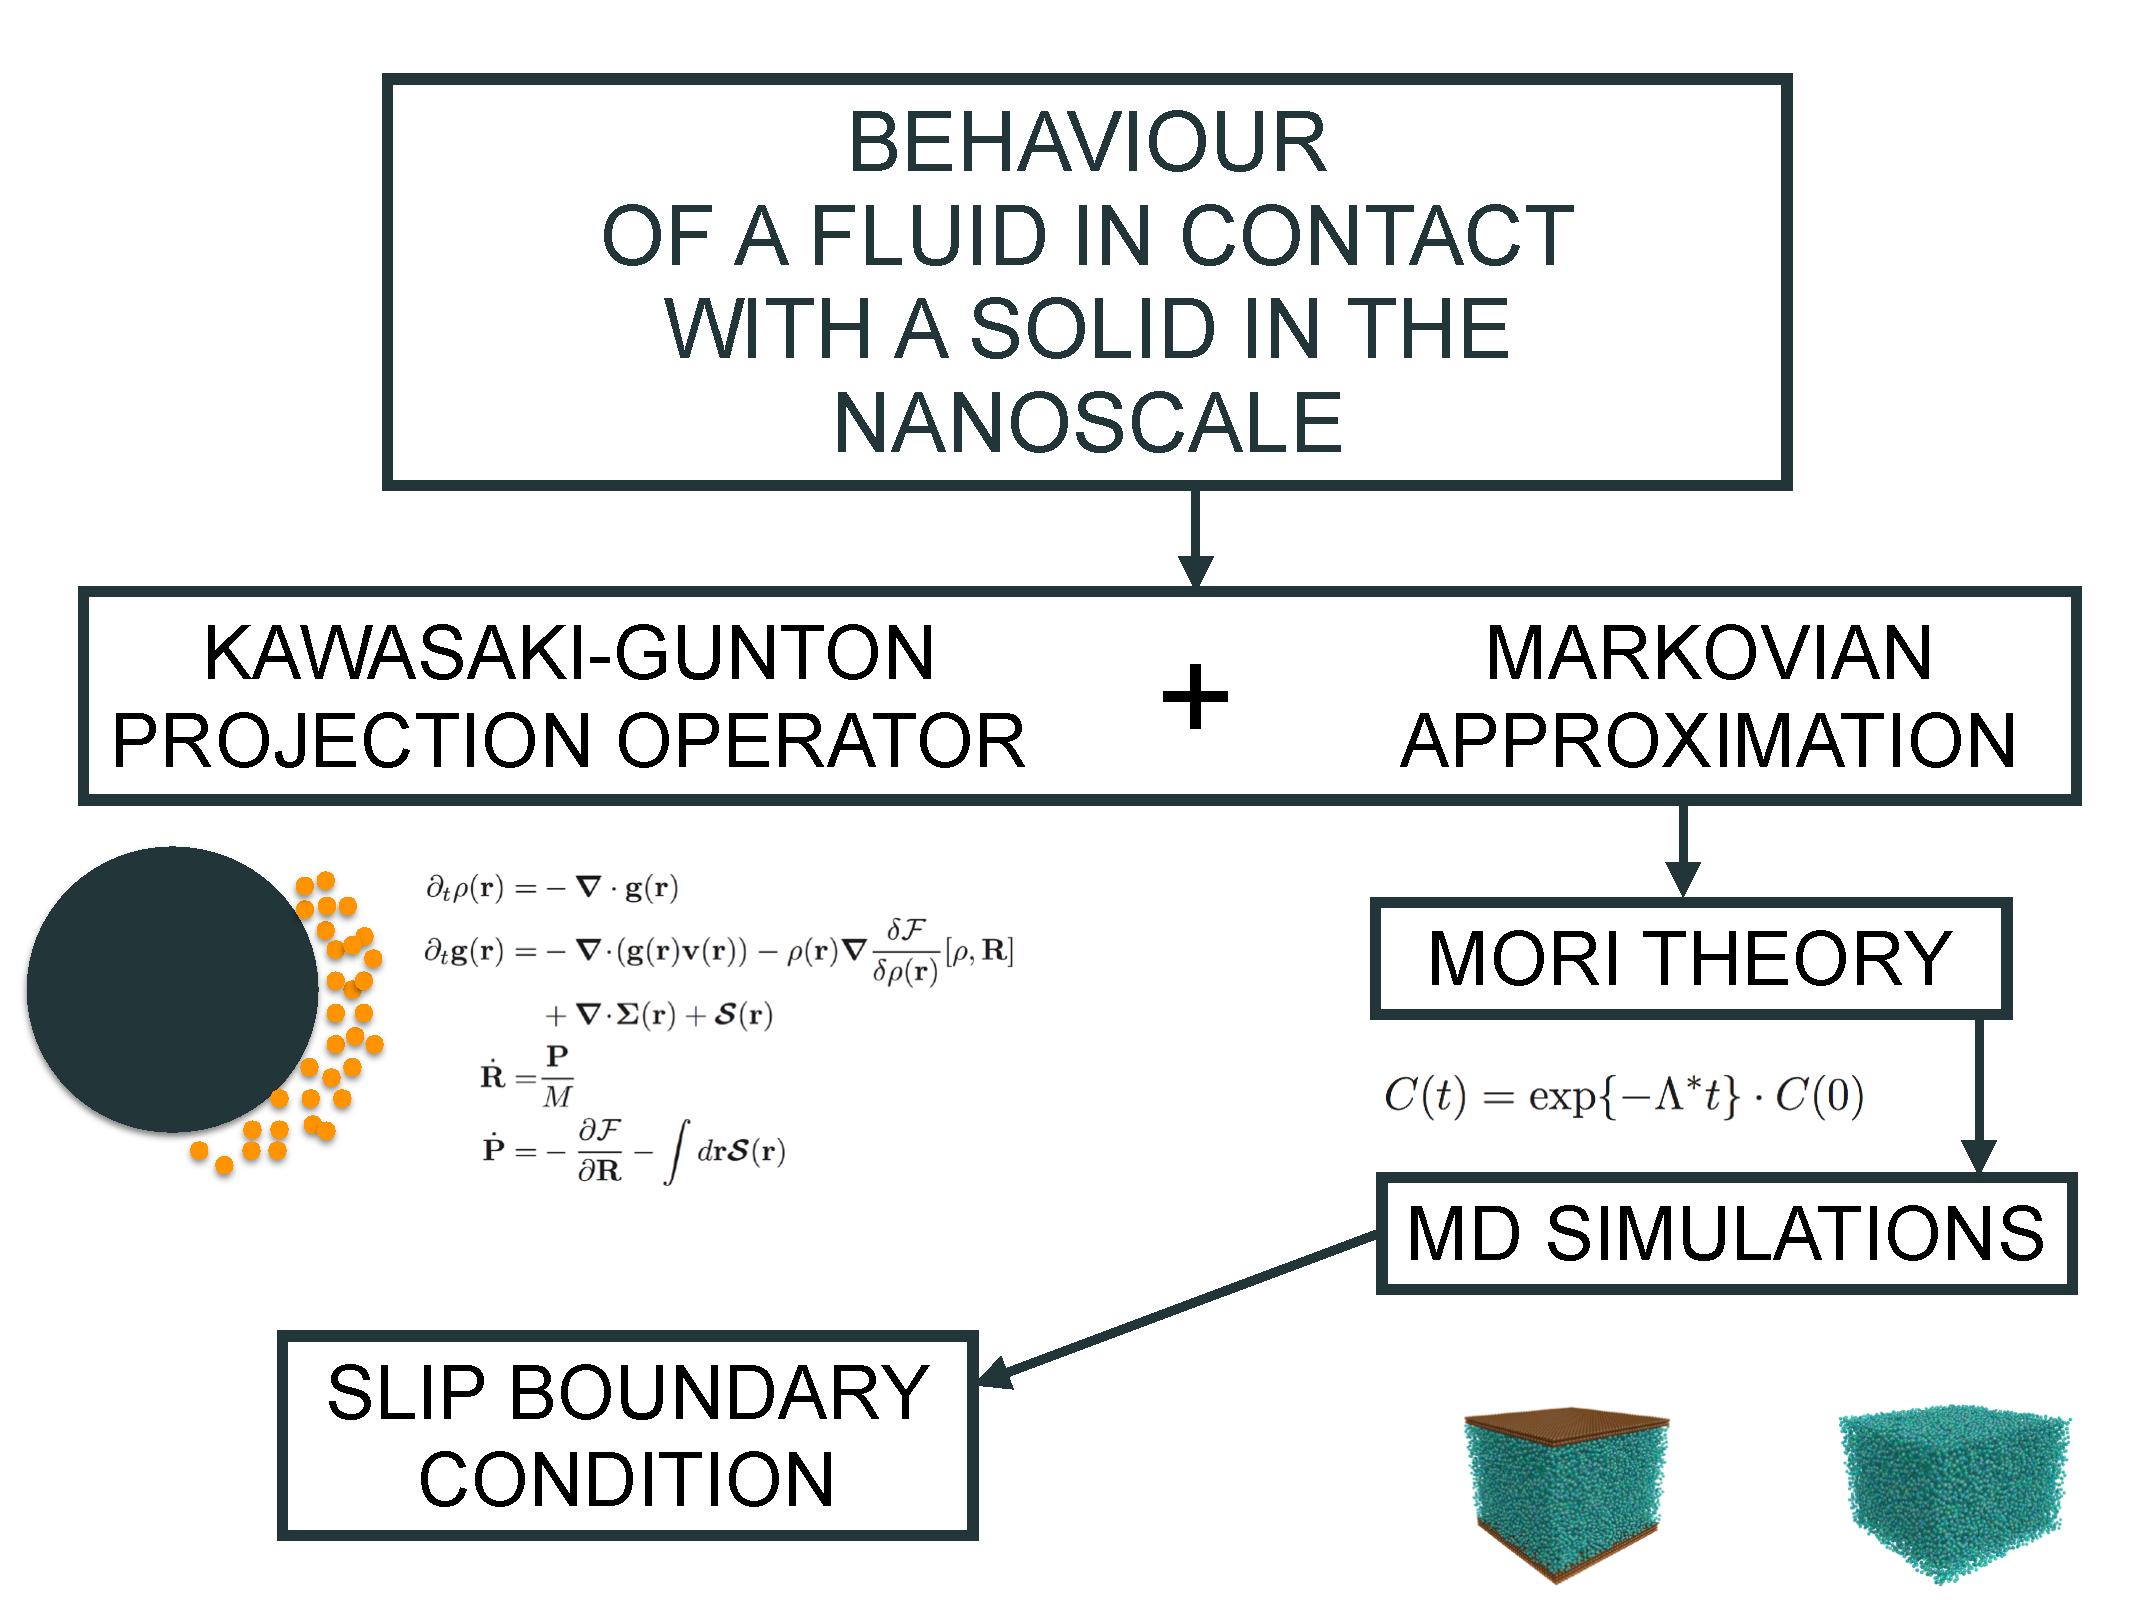
\includegraphics[width=\linewidth]{scheme-thesis}
\end{frame}

\begin{frame}{Derivation of the slip boundary condition}
\begin{itemize}
\item Through the  measurement of the correlation of
the  transverse  momentum  and  comparison  with  the  predictions  of
continuum  (local) hydrodynamics  \cite{Bocquet1993,Chen2015}.
\item Through
linear  response theory  relating  the  force on  the  walls with  the
velocity   of  the   fluid   \cite{Bocquet1993,Petravic2007}.
\item By formulating  linear,  in  general  non-Markovian,  conections  between
friction forces and velocities \cite{Hansen2011}, where the meaning of
this quantities is often understood implicitly.
\end{itemize}
\end{frame}

\begin{frame}{The slip problem from first principles}
  \begin{itemize}
\item Hydrodynamic equations from the microscopic dynamics of a fluid \cite{Piccirelli1968}.
\item Molecular Dynamics simulations in order to measure the transport coefficients that appear in the hydrodynamic equations in order to validate the theory.
\item The slip boundary condition is measured from a microscopic definition of the slip lenght and the position of the atomic wall. 
\end{itemize}
\end{frame}

\section{Nonequilibrium Statistical Mechanics}
\begin{frame}{The Theory of Coarse-Graining (ToCG)}
\begin{itemize}
\item The ToCG consists on eliminate the ``useless'' information about a system. 
\item Coarse grained (CG) variables.
%Selected variables with timescales much larger tha the typical molecular scales. 
\item Levels of description depending on the amount of information which one retains macroscopically.
  \begin{itemize}
    \item Macroscopic level.
    \item Microscopic level.
    \item Mesoscopic level.
    \end{itemize}
\end{itemize}
\end{frame}

\begin{frame}{The dynamics}
  \begin{itemize}
    %\item Set of CG variables $\hat{A}_i(z)$ and their averages $a_i(z)$
%\begin{align}
%    a = {\rm Tr}[{\hat{A}}\rho]
%    \nonumber
%\end{align}
    \item The aim is to \alert{derive equations of motion} for the time dependent average $a_i(t)$ of the CG variables $\hat{A}_i(z)$
      \begin{align}
        a_i(t)={\rm Tr}\left[\hat{A}_i(z)\rho_t\right]
        \nonumber
      \end{align}
    \item The trace symbol is given by
\begin{align}
  {\rm Tr}\left[\cdots\right]&=\sum_{N=0}^\infty \frac{1}{N!h^{3N}}
\int dzdz'\cdots \nonumber
\end{align}
\item $\rho_t$ is the nonequilibrium solution of the Liouville equation
\begin{align}
    \rho_t(z) = {\rm exp}\{-i{\cal L}t\}\rho_0(z)
    \nonumber
\end{align}
  \end{itemize}
\end{frame}

\begin{frame}{The dynamics. The Kawasaki-Gunton projection operator}
    For isolated systems with a time-independet Hamiltonian,the averages evolves according to the following equation \cite{Grabert1982}
      \begin{equation}
\frac{\partial }{\partial t} a_i(t)
= v_i(t) + \int_0^t dt' \sum_j K_{ij}(t,t') \lambda_j(t')
\nonumber
\end{equation}
\end{frame}

\begin{frame}{Kawasaki-Gunton projection operator. The reversible term}
\begin{itemize}
  \item The reversible term is given by
\begin{equation}
  v_i(t) = {\rm Tr}[\overline{\rho}_t  i{\cal L} \hat{A}_i]
  \nonumber
\label{vit}
\end{equation}
where $i{\cal L}$ is the Liouville operator and $\overline{\rho}_t$ is the \alert{relevant ensemble} which maximizes the Gibbs-Jaynes entropy functional
\begin{align}
 {\cal S}[\rho]&=-{\rm Tr}\left[\rho\ln\frac{\rho}{\rho_0}\right]
\nonumber
\label{entropy}
\end{align}

\item The form of $\overline{\rho}_t$ is
\begin{equation}
\overline{\rho}(z) = \frac{1}{Z[\lambda]} \rho_0\exp\{-\lambda\!\cdot\!\hat{A}(z)\}
\nonumber
\end{equation}
where $Z[\lambda]$ is the partition function and $\rho_0=\frac{1}{N!h^{3N}}$,   with  $h$  being   the  Planck's constant.
\end{itemize}
\end{frame}

\begin{frame}{Kawsaki-Gunton projection operator. The irreversible term}
\begin{itemize}
    \item The irreversible
      term involves the \alert{memory kernel}
\begin{equation}
K_{ij}(t,t') =
{\rm Tr}\left[\overline{\rho}_{t'} 
  \left({\cal Q}_{t'} i{\cal L}\hat{A}_j\right) G_{t't}
\left({\cal Q}_{t } i{\cal L}\hat{A}_i\right)\right]
\nonumber
\label{ker}
\end{equation}
where   the  Kawasaki-Gunton   projection  operator   ${\cal  Q}_{t'}$
applied  to an  arbitrary  function
$\hat{F}(z)$ is
\begin{align}
  {\cal Q}_{t'}\hat{F}(z) &= \hat{F}(z)- {\rm Tr}[\overline{\rho}_{t'} \hat{F}]
-\sum_i(\hat{A}_i(z)-a_i(t'))\frac{\partial }{\partial a_i(t')}
{\rm Tr}[\overline{\rho}_{t'} \hat{F}]
\label{Q}
\nonumber
\end{align}

\item The time ordered projected propagator $G_{t't}$ is given by
\begin{align}
  G_{t't}&=1
+\sum_{n=1}^\infty \int_{t'}^tdt_1\cdots\int_{t'}^{t_{n-1}}dt_n
i{\cal L}{\cal Q}_{t_n}\cdots  i{\cal L}{\cal Q}_{t_1}
\nonumber\\
&\equiv T_+\exp\left\{\int_{t'}^t dt''  i{\cal L}{\cal Q}_{t''}\right\}
\nonumber
\end{align}
where $T_+$ ensures that the operators are ordered from left to right as time increases.
\end{itemize}
  
\end{frame}

\begin{frame}{Kawasaki-Gunton projection operator. Markovian equation}
  \begin{itemize}
     \item Clear separation of timescales between the evolution of the averages and the decay of the memory kernel 
\begin{equation}
  \frac{\partial}{\partial t}a_i(t) = v_i(t) + \sum_j D_{ij}(t) \lambda_j(t)
\label{ex2}
\nonumber
\end{equation}
\item The  dissipative matrix  is  given  by  the Green-Kubo  formula
\begin{equation}
D_{ij}(t)=\int_0^{\Delta t} dt'\left\langle 
{\cal Q}_t i{\cal L}\hat{A}_j\exp\{i{\cal L}t'\}{\cal Q}_t i{\cal L}\hat{A}_i
\right\rangle^{\lambda(t)}
\label{dij}
\nonumber
\end{equation}
\item $\left\langle\cdots\right\rangle$ denotes an equilibrium average.
\end{itemize}
\end{frame}

\begin{frame}{The dynamics. Mori theory}
    The \alert{Mori's exact Generalized Langevin equation} \cite{Mori1965} is
\begin{align}
  \frac{d}{dt}\hat{A}(t)= & -L\esc C^{-1}(0)\esc \hat{A} (t) 
  -\int_0^tdt'\Gamma(t-t')\esc  C^{-1}(0)\esc \hat{A} (t') +F^+(t)
\nonumber
\end{align}
where the following matrices have been introduced
\begin{align}
  L&=\langle \hat{A}i{\cal L}\hat{A}^T\rangle \nonumber \\
  C(0)&=\langle \hat{A}\hat{A}^T\rangle \nonumber \\
\Gamma(t)&=\langle F^+(t)F^{+T}(0)\rangle
\nonumber
\end{align}
\end{frame}

\begin{frame}{Mori theory. Projected forces and projection operator}
  \begin{itemize}
\item The projected forces are given by
\begin{align}
F^+(t)&= \exp\{{\cal Q}i{\cal L}t\} {\cal Q}i{\cal L}\hat{A}  
\nonumber
\end{align}
\item $F^+(t)$ have zero mean and are uncorrelted from preivous values of the CG variables
\begin{align}
\langle  F^+  (t)\rangle&=0  
\nonumber\\
\langle \hat{A} F^+ (t)\rangle&=0 \quad\quad t\ge 0
\nonumber
\end{align}
\item The projection operator ${\cal Q}$ is defined as ${\cal Q}=1-{\cal P}$
  where  ${\cal P}$  is \alert{Mori's  projector} whose  effect on  an arbitrary
phase function $\hat{F}(z)$ is
\begin{align}
  {\cal P}\hat{F}(z) = \langle \hat{F}\rangle+ \langle \hat{F}\hat{A}^T \rangle\esc  C^{-1}(0)\esc  \hat{A}(z)
\nonumber
\end{align}
\end{itemize}
\end{frame}
\begin{frame}{Mori theory. Correlations and averages}
  \begin{itemize}
    \item The equilibrium time  correlation matrix of the CG variables is 
\begin{align}
  C(t)&=  \llangle \hat{A}(t)\hat{A}^T\rrangle
\nonumber
\end{align}
\item \alert{Mori's equation for correlations}
\begin{align}
  \frac{d}{dt}C(t)&=-L\esc C^{-1}(0)\esc C(t)
-\int_0^tdt' \Gamma(t-t')\esc C^{-1}(0)\esc  C(t')
\nonumber
\end{align}

\item The time-dependent average of the CG variables is defined as
\begin{align}
  a(t)&=\int dz \rho_0(z) \exp\{i{\cal L}t\}\hat{A}(z)
  \nonumber
\end{align}
\item \alert{Mori's equation for averages}
\begin{align}
  \frac{d}{dt}a(t) = -L\esc C^{-1}(0)\esc a(t)
-\int_0^tdt' \Gamma(t-t')\esc  C^{-1}(0)\esc a(t')
\label{exactAve}
\nonumber
\end{align}
\end{itemize}
\end{frame}

\begin{frame}{Mori theory. Markovian aproximation}
  \begin{itemize}
    \item The linear integro-differential term can be approximated by a memory-less term
      \begin{align}
  \frac{d}{dt}C(t)&=-L\esc C^{-1}(0)\esc C(t)
  -\underbrace{\int_0^tdt' \Gamma(t-t')\esc C^{-1}(0)\esc  C(t')}_{M^* C^{-1}(0)C(t)}
\nonumber
\end{align}
\item Evolution equation for the correlations
\begin{align}
  \frac{d}{dt}C(t)&=-(L+M^*)C^{-1}(0)C(t) 
  \nonumber \\
  &= \Lambda^*\esc  C(t)
\nonumber
\end{align}
\item The \alert{relaxation matrix} $\Lambda^*$ is defined as
\begin{align}
\Lambda^*\equiv(L+M^*)\esc C^{-1}(0)  
\nonumber
\end{align}
\end{itemize}
\end{frame}

\begin{frame}{Mori theory. Markovian aproximation}
  \begin{itemize}
    \item  The only possibility for a correlation is to \alert{decay in an exponential matrix way} 
\begin{align}
  C(t)=\exp\{-\Lambda^* t\}\esc C(0)
\nonumber
\end{align}
\item At short times 
\begin{align}
    \frac{d}{dt}C(0)&=-L
  \nonumber
\end{align}
which is only possible if $M^*=0$.
\item The correlations  will decay  in an
  exponential (Markovian)  way only  after the  time $\tau$  beyond which
memory is lost. 
\begin{align}
  C(t)=\exp\{-\Lambda^* (t-\tau)\}\esc C(\tau)
\nonumber
\end{align}
\end{itemize}
\end{frame}

\begin{frame}{Summary}
  \begin{itemize}
    \item Kawasaki-Gunton and Mori theory. 
    \item Exponential decay of the matrix of correlations after a time $\tau$.
    \end{itemize}
\end{frame}

\section{Continuum hydrodynamics theory for liquids near solids}
\end{document}
